\documentclass{article}
\usepackage{amsmath}
\usepackage{color,pxfonts,fix-cm}
\usepackage{latexsym}
\usepackage[mathletters]{ucs}
\DeclareUnicodeCharacter{32}{$\ $}
\usepackage[T1]{fontenc}
\usepackage[utf8x]{inputenc}
\usepackage{pict2e}
\usepackage{wasysym}
\usepackage[english]{babel}
\usepackage{tikz}
\pagestyle{empty}
\usepackage[margin=0in,paperwidth=596pt,paperheight=843pt]{geometry}
\begin{document}
\definecolor{color_283006}{rgb}{1,1,1}
\definecolor{color_29791}{rgb}{0,0,0}
\begin{tikzpicture}[overlay]
\path(0pt,0pt);
\filldraw[color_283006][nonzero rule]
(-15pt, 10pt) -- (581pt, 10pt)
 -- (581pt, 10pt)
 -- (581pt, -832.9572pt)
 -- (581pt, -832.9572pt)
 -- (-15pt, -832.9572pt) -- cycle
;
\filldraw[color_283006][nonzero rule]
(-15pt, 10pt) -- (581pt, 10pt)
 -- (581pt, 10pt)
 -- (581pt, -832.9572pt)
 -- (581pt, -832.9572pt)
 -- (-15pt, -832.9572pt) -- cycle
;
\filldraw[color_283006][nonzero rule]
(-15pt, 10pt) -- (581pt, 10pt)
 -- (581pt, 10pt)
 -- (581pt, -2518.872pt)
 -- (581pt, -2518.872pt)
 -- (-15pt, -2518.872pt) -- cycle
;
\filldraw[color_283006][nonzero rule]
(-15pt, 10pt) -- (581pt, 10pt)
 -- (581pt, 10pt)
 -- (581pt, -832.9572pt)
 -- (581pt, -832.9572pt)
 -- (-15pt, -832.9572pt) -- cycle
;
\filldraw[color_283006][nonzero rule]
(-15pt, -62.06042pt) -- (581pt, -62.06042pt)
 -- (581pt, -62.06042pt)
 -- (581pt, -832.9572pt)
 -- (581pt, -832.9572pt)
 -- (-15pt, -832.9572pt) -- cycle
;
\end{tikzpicture}
\begin{picture}(-5,0)(2.5,0)
\put(577.2468,-504.932){\fontsize{11.00423}{1}\usefont{T1}{uarial}{m}{n}\selectfont\color{color_29791} }
\put(-11.62238,-505.3076){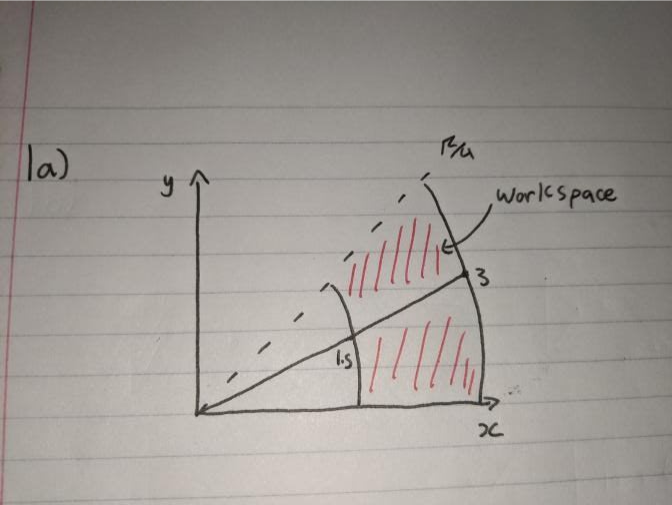
\includegraphics[width=587.7435pt,height=441.3709pt]{latexImage_6557208db40ade990d779d85beafa477.png}}
\end{picture}
\newpage
\begin{tikzpicture}[overlay]
\path(0pt,0pt);
\filldraw[color_283006][nonzero rule]
(-15pt, 10pt) -- (581pt, 10pt)
 -- (581pt, 10pt)
 -- (581pt, -832.9572pt)
 -- (581pt, -832.9572pt)
 -- (-15pt, -832.9572pt) -- cycle
;
\filldraw[color_283006][nonzero rule]
(-15pt, 10pt) -- (581pt, 10pt)
 -- (581pt, 10pt)
 -- (581pt, -832.9572pt)
 -- (581pt, -832.9572pt)
 -- (-15pt, -832.9572pt) -- cycle
;
\filldraw[color_283006][nonzero rule]
(-15pt, 852.9572pt) -- (581pt, 852.9572pt)
 -- (581pt, 852.9572pt)
 -- (581pt, -1675.914pt)
 -- (581pt, -1675.914pt)
 -- (-15pt, -1675.914pt) -- cycle
;
\filldraw[color_283006][nonzero rule]
(-15pt, 10pt) -- (581pt, 10pt)
 -- (581pt, 10pt)
 -- (581pt, -832.9572pt)
 -- (581pt, -832.9572pt)
 -- (-15pt, -832.9572pt) -- cycle
;
\filldraw[color_283006][nonzero rule]
(-15pt, -62.06049pt) -- (581pt, -62.06049pt)
 -- (581pt, -62.06049pt)
 -- (581pt, -832.9572pt)
 -- (581pt, -832.9572pt)
 -- (-15pt, -832.9572pt) -- cycle
;
\end{tikzpicture}
\begin{picture}(-5,0)(2.5,0)
\put(541.9672,-802.932){\fontsize{11.00423}{1}\usefont{T1}{uarial}{m}{n}\selectfont\color{color_29791} }
\put(-567.0895,-803.3064){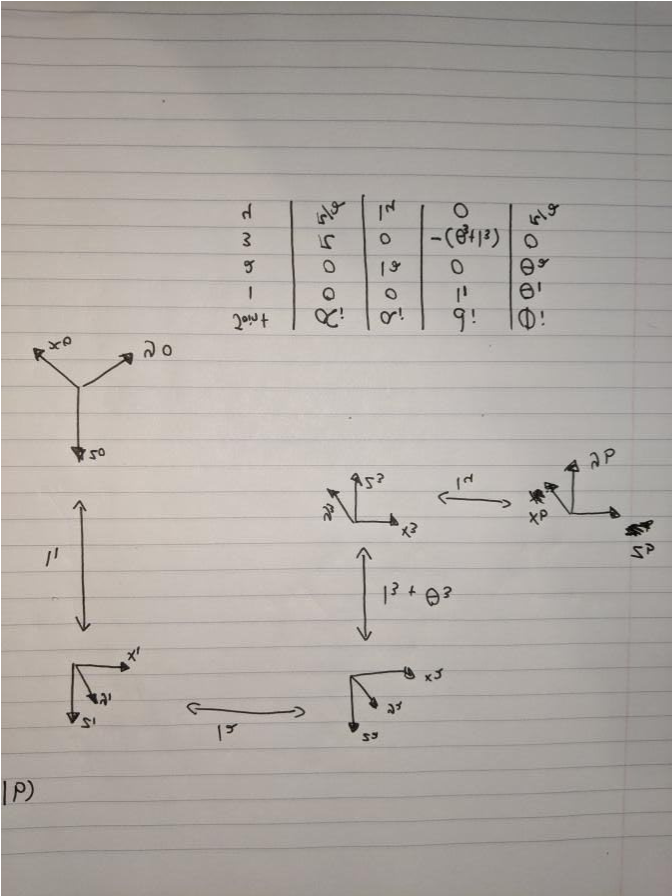
\includegraphics[width=553.9675pt,height=739.3724pt]{latexImage_75647e084e99157403ef8f82a86aec0f.png}}
\end{picture}
\newpage
\begin{tikzpicture}[overlay]
\path(0pt,0pt);
\filldraw[color_283006][nonzero rule]
(-15pt, 10pt) -- (581pt, 10pt)
 -- (581pt, 10pt)
 -- (581pt, -832.9573pt)
 -- (581pt, -832.9573pt)
 -- (-15pt, -832.9573pt) -- cycle
;
\filldraw[color_283006][nonzero rule]
(-15pt, 10pt) -- (581pt, 10pt)
 -- (581pt, 10pt)
 -- (581pt, -832.9573pt)
 -- (581pt, -832.9573pt)
 -- (-15pt, -832.9573pt) -- cycle
;
\filldraw[color_283006][nonzero rule]
(-15pt, 1695.914pt) -- (581pt, 1695.914pt)
 -- (581pt, 1695.914pt)
 -- (581pt, -832.9573pt)
 -- (581pt, -832.9573pt)
 -- (-15pt, -832.9573pt) -- cycle
;
\filldraw[color_283006][nonzero rule]
(-15pt, 10pt) -- (581pt, 10pt)
 -- (581pt, 10pt)
 -- (581pt, -832.9573pt)
 -- (581pt, -832.9573pt)
 -- (-15pt, -832.9573pt) -- cycle
;
\filldraw[color_283006][nonzero rule]
(-15pt, -62.06055pt) -- (581pt, -62.06055pt)
 -- (581pt, -62.06055pt)
 -- (581pt, -832.9573pt)
 -- (581pt, -832.9573pt)
 -- (-15pt, -832.9573pt) -- cycle
;
\end{tikzpicture}
\begin{picture}(-5,0)(2.5,0)
\put(57.06046,-71.81873){\fontsize{11.00423}{1}\usefont{T1}{uarial}{m}{n}\selectfont\color{color_29791} }
\put(57.06046,-86.8313){\fontsize{11.00423}{1}\usefont{T1}{uarial}{m}{n}\selectfont\color{color_29791} }
\put(578.7481,-534.9573){\fontsize{11.00423}{1}\usefont{T1}{uarial}{m}{n}\selectfont\color{color_29791} }
\put(-13.49939,-92.08496){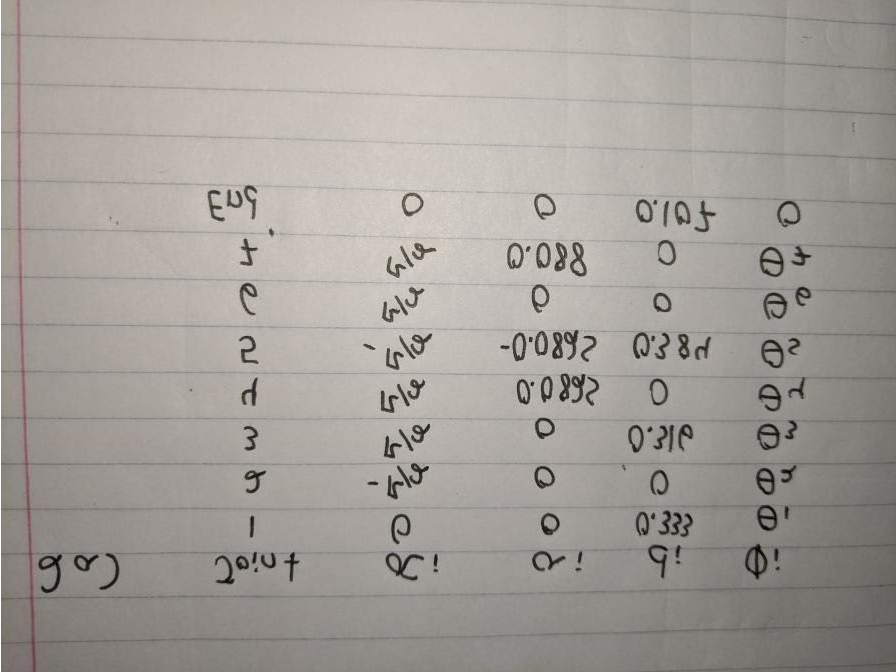
\includegraphics[width=590.7457pt,height=442.8716pt]{latexImage_b461805a06336aa4316762b57e2e532e.png}}
\end{picture}
\end{document}